%!TEX root = ../main.tex

\vspace{-1em}

% =================================================

\section{\color{red}Costitutive Classes}

% =================================================

\textbf{Change of frame/observer.} It is just a \emph{superposed rigid body motion} $\chi^*(p,t)=r\circ \chi$, where the motion $\chi$ is
\begin{equation*}
\chi(p,t)-\chi(q,t)=F(p,t)[p-q]
\end{equation*}

and the rigid motion $r$ is
\begin{equation*}
r(x,t)-r(y,t)=Q(t)[x-y]
\end{equation*}

with $Q(t)\in\text{SO}(3)$ called \emph{frame-rotation}, and $\Omega=\dot{Q}Q^T\in\text{Skw}$ called \emph{frame-spin}.
\vspace{-0.5em}
\begin{Figure}
    \center{
    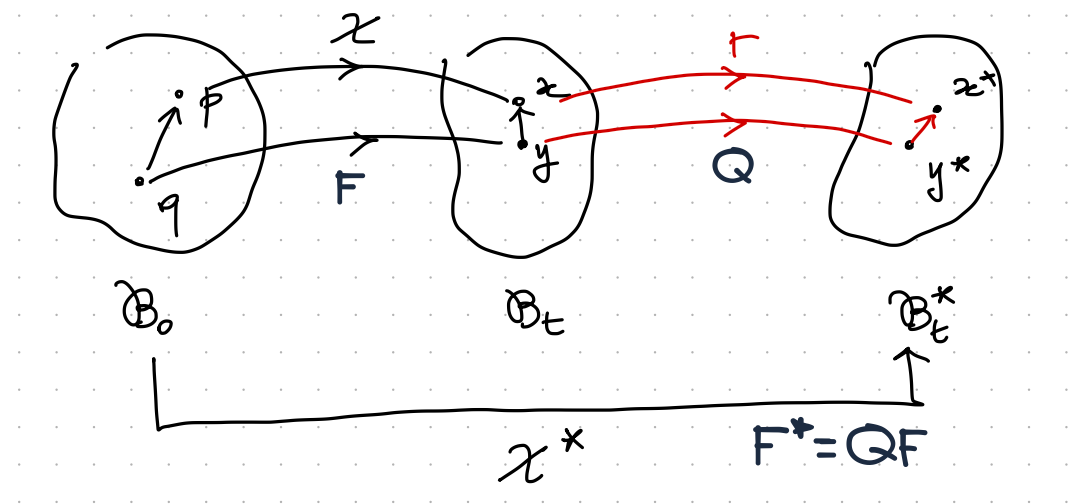
\includegraphics[width=0.7\linewidth]{images/def4}\ \ }
\end{Figure}
\vspace{-0.5em}
$\leadsto \chi^*(p,t)-\chi^*(q,t)=F^*(p,t)[p-q],\,\boxed{F^*=QF}$

\smallskip

In general, we can prove the followings:
\begin{equation*}
\begin{array}{ll}
C^*=C & B^*=QBQ^T \\
T^*=QTQ^T & S^*=QS \\
L^*=\Omega+QLQ^T & D^*=QDQ^T \\ 
&W^*=\Omega+QWQ^T \\
\end{array} \tag{$\circledast$}
\end{equation*}

\textbf{\color{lavender(floral)}Proof.} See whiteboard 5 u.u

\smallskip

\textbf{Rmk:} by $(\circledast)$, one can call $C$ \emph{invariant} and $B,T,D$ \emph{frame-indifferent} or \emph{objective}.

\rule{0.31\textwidth}{0.2pt}
\smallskip

\textbf{Def.} $(\chi,T)$ is a \emph{mechanical process}. A \emph{costitutive class} $\Cc$ is a subset (i.e. a restriction) of the whole set of mechanical processes.

\rule{0.31\textwidth}{0.2pt}
\smallskip

\textbf{Principle of frame indifference (PFI).} "Physical laws be independent of the frame of reference", in other words
\begin{equation*}
(\chi,T)\in\Cc\ \Longleftrightarrow\ (\chi^*,T^*)\in\Cc  
\end{equation*}

where $\chi^*,\ T^*$ are obtained by superposed rbm.

\rule{0.31\textwidth}{0.2pt}
\smallskip

\textbf{Material simmetry.} Let $\ti$ be a costitutive law, i.e. $T=\ti(F)$. We call
\begin{equation*}
\Gc=\left\{ H\in\text{Lin}^+\,:\,\ti(FH)=\ti(F)\ \forall\, F\in \text{Lin}^+ \right\}
\end{equation*}
the \emph{symmetry group} of the body ($\Gc$ is a group, i.e. $I\in \Gc,\ H_1,H_2,H_3\in \Gc\,\Rightarrow\,H_1H_2,H_3^{\text{-}1}\in \Gc$) \\ $\leadsto$ there are no privileged stress directions.

\smallskip 

To avoid phisically unacceptable situations (when you deform a body in a single point or you make it infinitely big) we set $\text{det}(H)=1$, i.e.
\begin{equation*}
\Gc=\left\{ H\in\text{SL}(3)\,:\,\ti(FH)=\ti(F)\ \forall\, F\in \text{Lin}^+ \right\}
\end{equation*}

\textbf{Thm.} Every $G$ st $\text{SL}(3)\subseteq G \subseteq \text{SO}(3)$ must either be $G=\text{SL}(3)$ or $G=\text{SO}(3)$ (there are no isotropic materials \emph{between} solids and fluids).

\smallskip

We'll consider $G=\text{SL}(3)$ (fluids), $G\supseteq\text{SO}(3)$ (isotropic materials), $G\subseteq \text{SO}(3)$ (solids), $G=\text{SO}(3)$ (isotropic solids).   

\rule{0.31\textwidth}{1pt}

